\documentclass[10pt,twocolumn]{article}
\usepackage[margin=0.65in]{geometry}
\usepackage{booktabs}
\usepackage{graphicx}
\usepackage{hyperref}
\usepackage{xurl}
\usepackage{microtype}
\usepackage{amsmath}
\usepackage{caption}
\captionsetup{font=small,labelfont=bf}
\hypersetup{colorlinks=true,urlcolor=blue,citecolor=blue,linkcolor=blue}

\title{Clinical and Hormonal Predictors of BMI in Women with PCOS: Statistical First Run}
\author{Soumitra Das \and Shreya Saha \and Anjali Kanvinde \and Shivraj Singh Bhatti \and Pranav Jeyakumar}
\date{\today}

\begin{document}
\sloppy
\maketitle

\begin{abstract}
We analyze the Kaggle PCOS dataset by Prasoon Kottarathil, with 541 records and 177 PCOS-positive participants. The response variable is BMI. This first run uses descriptive statistics, scatterplots, Pearson correlation, simple linear regression, a Welch two-sample t-test, one-way ANOVA, multiple linear regression, adjusted $R^2$, VIF values, residual plots, and sensitivity checks. Fasting insulin and testosterone were not present in the downloaded workbook, so we use available clinical, hormonal, lifestyle, and ultrasound variables.
\end{abstract}

\section{Research Question and Data}
Our question is: among women with PCOS, which clinical, hormonal, lifestyle, and ultrasound variables are associated with BMI? The main analysis is restricted to PCOS-positive participants ($n=177$). We also include a short PCOS vs non-PCOS context table to understand how the analytic subset differs from the rest of the dataset.

\section{Community and Research Motivation}
The Kaggle dataset page reports substantial public use, including code notebooks and discussions: \url{https://www.kaggle.com/datasets/prasoonkottarathil/polycystic-ovary-syndrome-pcos}. Recent work using this same dataset groups variables into clinical, laboratory, and ultrasound blocks and studies BMI/cycle subgroups \cite{autopcos}. Explainable-machine-learning work using this dataset highlights follicle counts, AMH, weight gain, skin darkening, hair growth, and FSH/LH-related variables as important for PCOS classification \cite{mdpi}. A recent preprint also notes that the Kaggle diagnosis label lacks verifiable diagnostic criteria, so our results should be framed as exploratory rather than clinical proof \cite{medrxiv}.

\section{Descriptive Statistics}
Among PCOS-positive participants, mean BMI was 25.47 with standard deviation 4.40; the median was 25.10. BMI skewness was 0.232, so BMI was not extremely skewed in this subset. Mean AMH was 7.84, and mean waist-to-hip ratio was 0.893.

\begin{figure}[t]
\centering
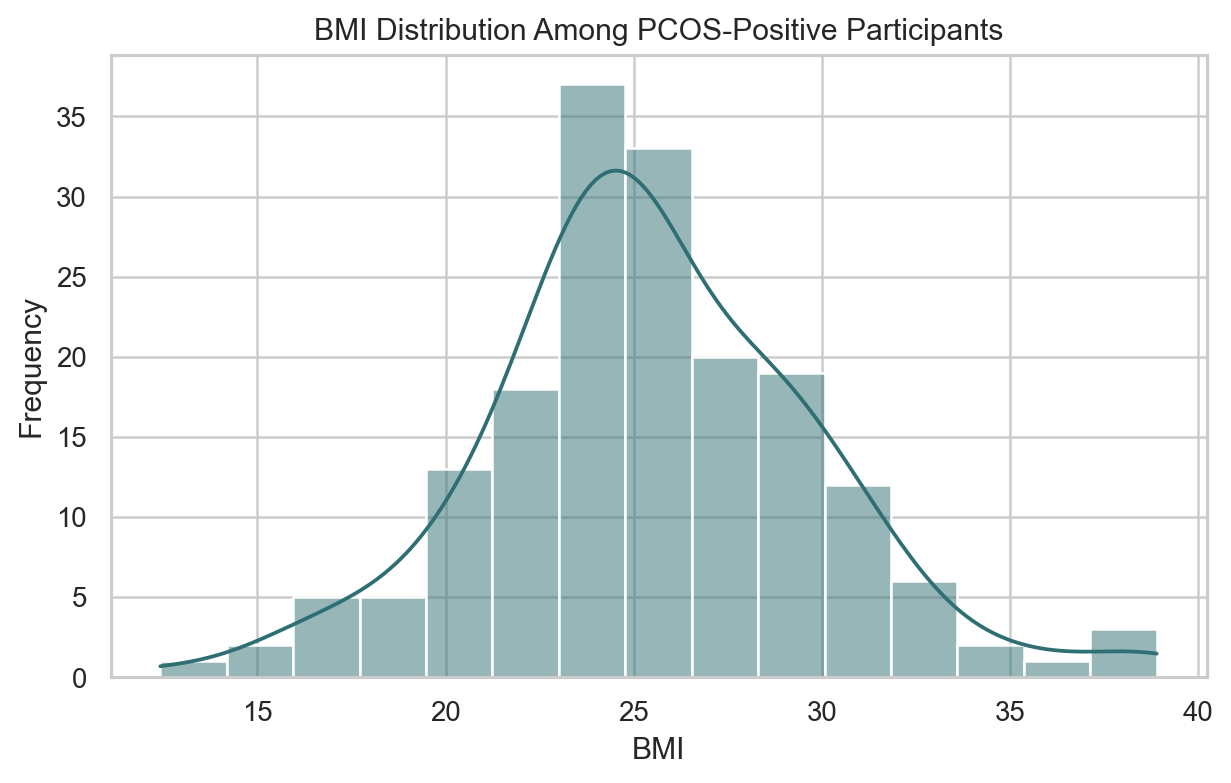
\includegraphics[width=\columnwidth]{../figures/bmi_distribution.png}
\caption{BMI distribution among PCOS-positive participants.}
\end{figure}

\section{Simple Linear Regression}
The simple linear regression used BMI as the response variable and waist-to-hip ratio as the explanatory variable. Pearson correlation was $r=0.084$ with $p=0.2678$. The slope estimate was 7.93 BMI units per 1.0 waist-to-hip-ratio unit, but this association was not statistically significant ($p=0.2678$), and $R^2=0.007$.

\begin{figure}[t]
\centering
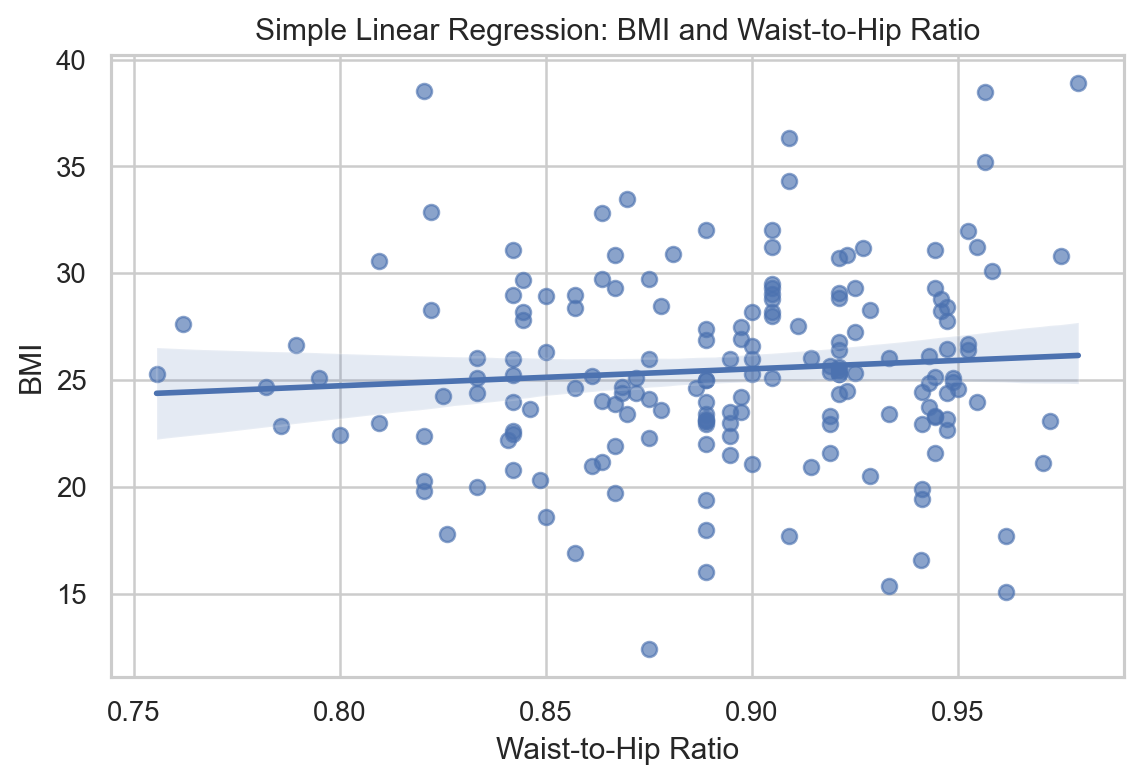
\includegraphics[width=\columnwidth]{../figures/bmi_vs_waist_hip_ratio.png}
\caption{Scatterplot with least-squares regression line for BMI and waist-to-hip ratio.}
\end{figure}

\section{Two-Sample t-Test and ANOVA}
Mean BMI was 26.28 for irregular cycles and 24.53 for regular cycles. A Welch two-sample t-test gave $t=-2.70$ and $p=0.0076$, suggesting higher BMI among participants with irregular cycles before adjustment.

\begin{figure}[t]
\centering
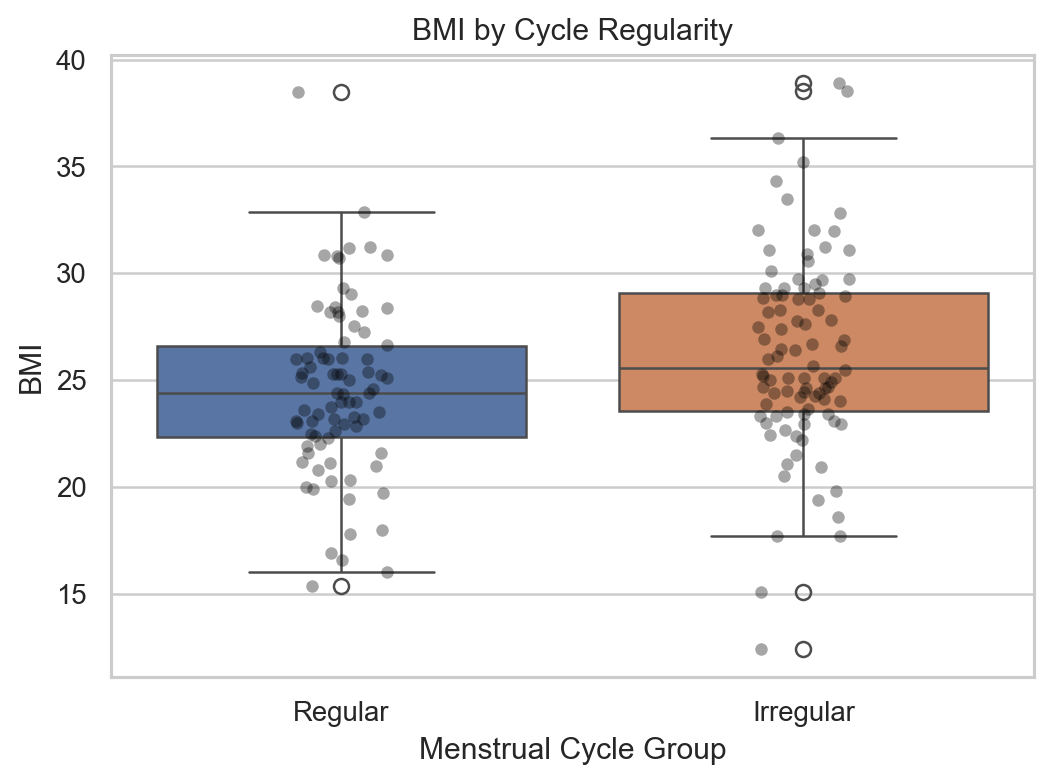
\includegraphics[width=\columnwidth]{../figures/bmi_by_cycle_group.png}
\caption{BMI by menstrual cycle regularity.}
\end{figure}

For the one-way ANOVA, we split total follicle count into low, medium, and high groups. The ANOVA was not statistically significant, $F=0.10$, $p=0.9039$, so Tukey's HSD was not needed.

\begin{figure}[t]
\centering
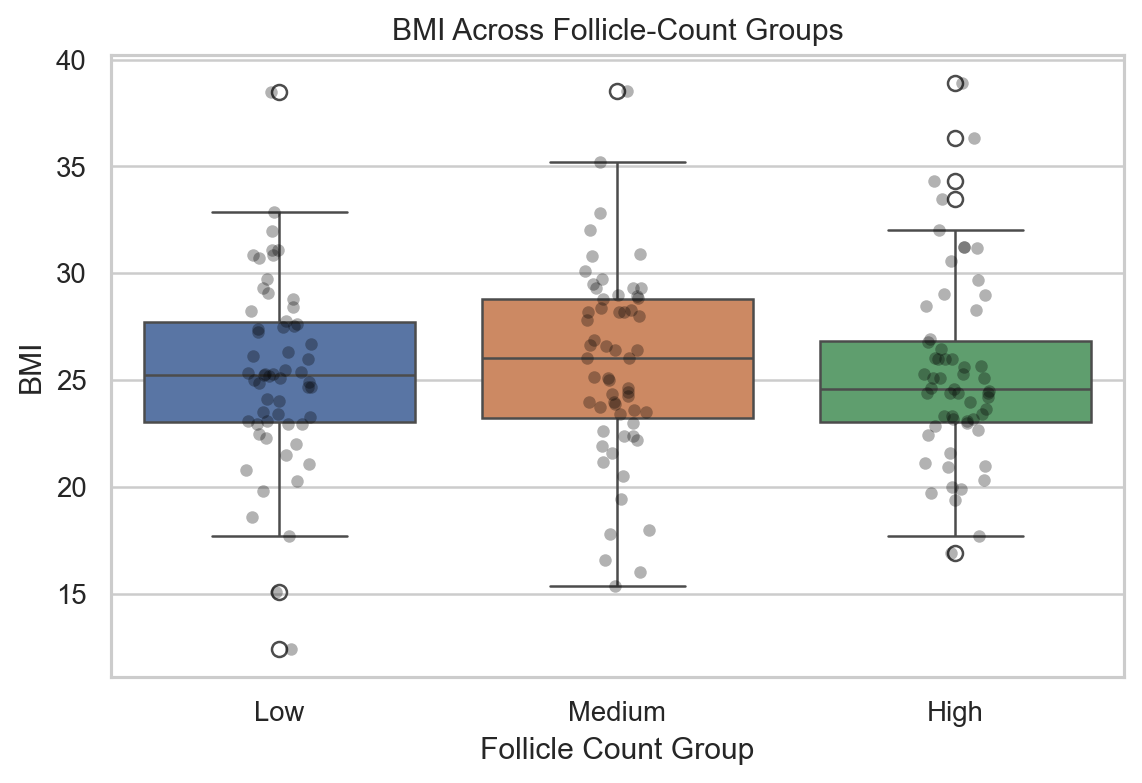
\includegraphics[width=\columnwidth]{../figures/bmi_by_follicle_group.png}
\caption{BMI across low, medium, and high follicle-count groups.}
\end{figure}

\section{Multiple Regression}
The full multiple linear regression included clinical, hormonal, lifestyle, and ultrasound predictors. The full model adjusted $R^2$ was 0.237; the reduced clinical model adjusted $R^2$ was 0.260. VIF values for non-intercept predictors were all close to 1, suggesting no major multicollinearity problem.

\begin{table}[t]
\caption{Largest full-model terms by absolute t-statistic.}
\label{tab:coef}
\small\resizebox{\columnwidth}{!}{\begin{tabular}{lrrl}
\toprule
Term & Estimate & SE & p \\
\midrule
weight\_gain & 4.321 & 0.686 & $<0.001$ \\
waist\_hip\_ratio & 11.341 & 6.969 & 0.106 \\
fast\_food & 0.965 & 0.770 & 0.212 \\
age & 0.072 & 0.061 & 0.237 \\
C(cycle\_group)[T.Regular] & -0.653 & 0.617 & 0.291 \\
tsh & 0.102 & 0.104 & 0.331 \\
regular\_exercise & -0.352 & 0.698 & 0.614 \\
lh\_fsh\_ratio & 0.004 & 0.009 & 0.671 \\
\bottomrule
\end{tabular}}
\end{table}


\section{Model Block Comparison}
Following the structure used in recent community/research modeling, we compared clinical-only, laboratory-only, ultrasound-only, and combined model blocks using adjusted $R^2$. This asks whether easy-to-collect clinical variables explain BMI about as well as more intensive hormone or ultrasound variables.

\begin{figure}[t]
\centering
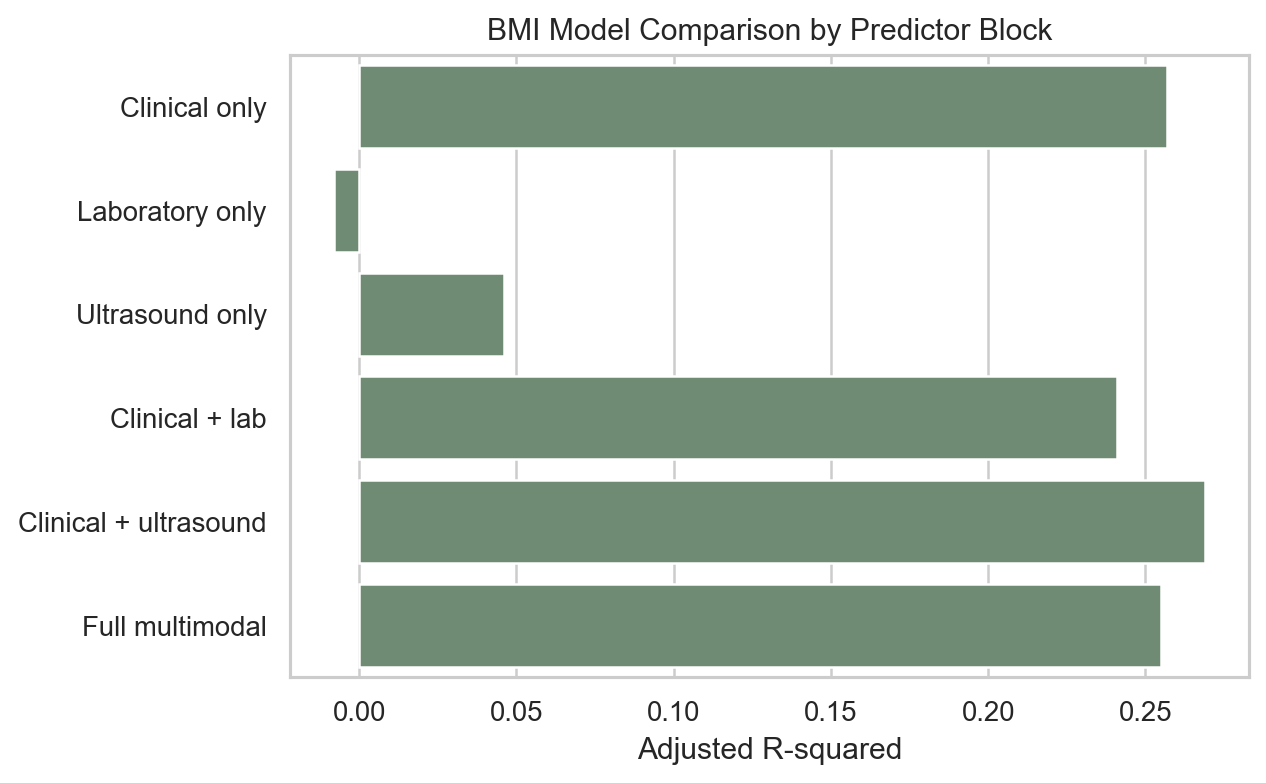
\includegraphics[width=\columnwidth]{../figures/model_block_adjusted_r2.png}
\caption{Adjusted $R^2$ by predictor block.}
\end{figure}

\begin{table}[t]
\caption{Adjusted $R^2$ comparison by predictor block.}
\label{tab:block}
\small\resizebox{\columnwidth}{!}{\begin{tabular}{lrrr}
\toprule
Model block & n & Adj. R2 & AIC \\
\midrule
Clinical only & 176 & 0.257 & 976.200 \\
Laboratory only & 176 & -0.008 & 1029.000 \\
Ultrasound only & 176 & 0.046 & 1019.300 \\
Clinical + lab & 176 & 0.241 & 984.700 \\
Clinical + ultrasound & 176 & 0.269 & 978.000 \\
Full multimodal & 176 & 0.255 & 986.000 \\
\bottomrule
\end{tabular}}
\end{table}


\section{BMI Subgroup Checks}
Because recent work stratifies by BMI $<24$ vs BMI $\geq 24$, we used the same threshold as an exploratory subgroup check. Since BMI defines the groups, these results should be interpreted as descriptive comparisons of associated variables rather than causal tests.

\begin{figure}[t]
\centering
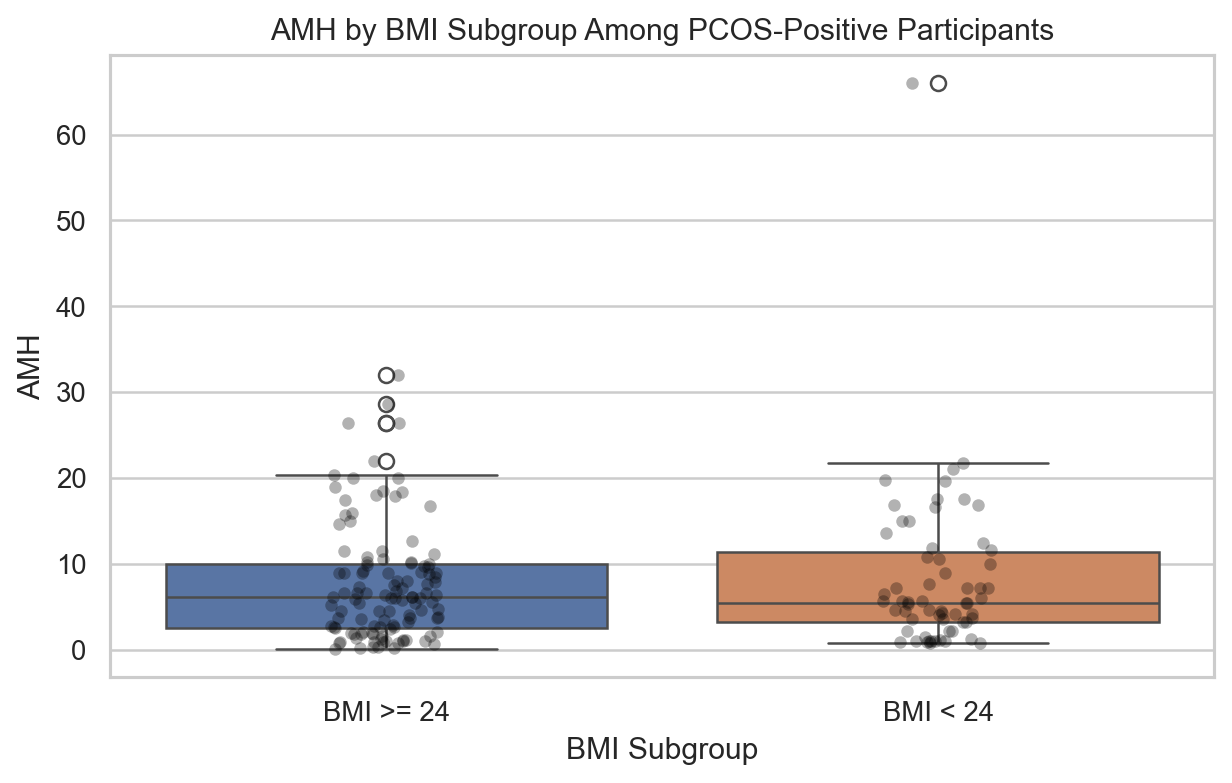
\includegraphics[width=\columnwidth]{../figures/amh_by_bmi_subgroup.png}
\caption{AMH by BMI subgroup among PCOS-positive participants.}
\end{figure}

\begin{table}[t]
\caption{Exploratory BMI subgroup comparisons among PCOS-positive participants.}
\label{tab:subgroup}
\small\resizebox{\columnwidth}{!}{\begin{tabular}{lrrl}
\toprule
Variable & BMI < 24 mean & BMI >= 24 mean & p \\
\midrule
AMH & 8.265 & 7.618 & 0.637 \\
Waist:hip ratio & 0.890 & 0.894 & 0.523 \\
Total follicles & 21.226 & 20.183 & 0.399 \\
RBS & 99.242 & 102.158 & 0.356 \\
\bottomrule
\end{tabular}}
\end{table}


\section{PCOS vs Non-PCOS Context}
Although our main response is BMI among PCOS-positive participants, this table helps the team understand what separates the PCOS-positive and non-PCOS rows in the dataset.

\begin{figure}[t]
\centering
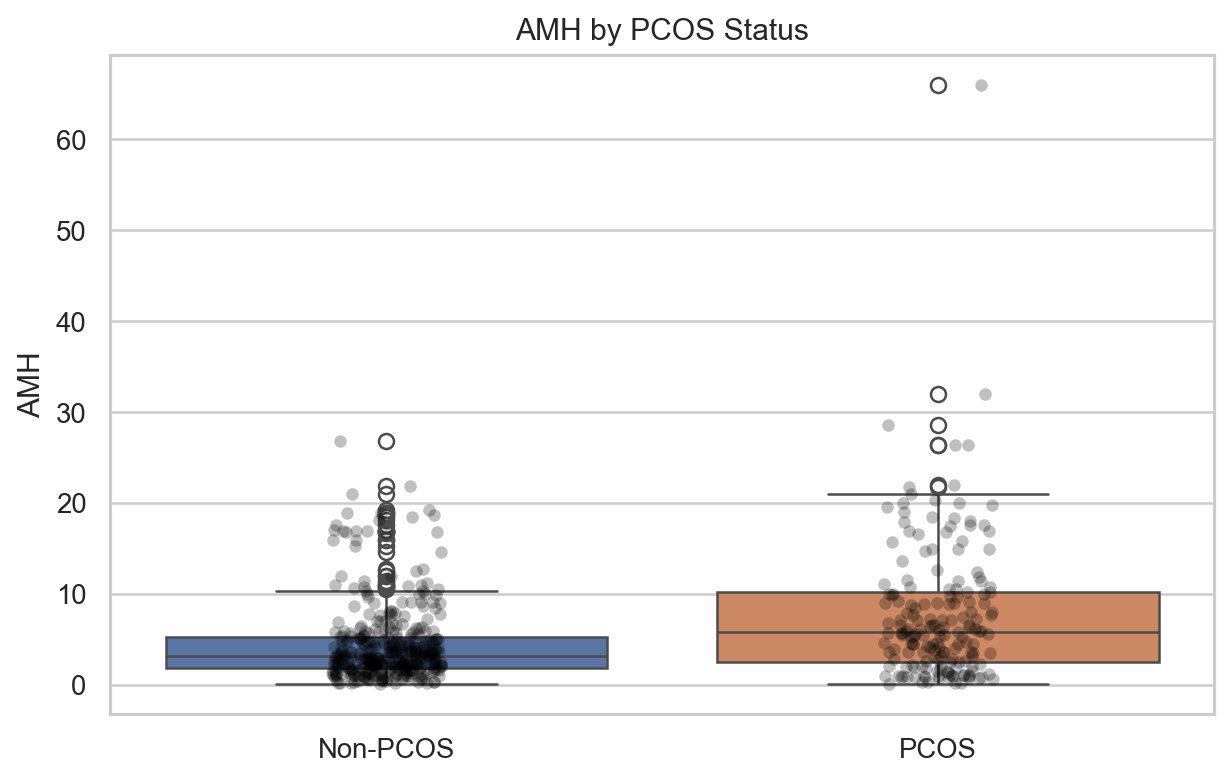
\includegraphics[width=\columnwidth]{../figures/amh_by_pcos_status.png}
\caption{AMH by PCOS status in the full dataset.}
\end{figure}

\begin{table}[t]
\caption{Exploratory PCOS vs non-PCOS context comparisons.}
\label{tab:context}
\small\resizebox{\columnwidth}{!}{\begin{tabular}{lrrl}
\toprule
Variable & PCOS mean & Non-PCOS mean & p \\
\midrule
BMI & 25.471 & 23.747 & $<0.001$ \\
AMH & 7.845 & 4.541 & $<0.001$ \\
Waist:hip ratio & 0.893 & 0.891 & 0.774 \\
Total follicles & 20.548 & 8.989 & $<0.001$ \\
Weight gain & 0.684 & 0.228 & $<0.001$ \\
Fast food & 0.785 & 0.383 & $<0.001$ \\
Irregular cycle & 0.531 & 0.154 & $<0.001$ \\
\bottomrule
\end{tabular}}
\end{table}


\section{Interactions and Sensitivity Checks}
We tried a small set of theory-informed interaction terms and sensitivity checks. The goal is not stepwise selection; it is to see whether the main conclusions are stable when we allow simple effect modification or reduce the influence of extreme hormone/BMI values.

\begin{table}[t]
\caption{Interaction model comparison.}
\label{tab:interactions}
\small\resizebox{\columnwidth}{!}{\begin{tabular}{lrrr}
\toprule
Model & n & Adj. R2 & AIC \\
\midrule
Clinical base & 176 & 0.257 & 976.200 \\
Cycle x weight gain & 176 & 0.261 & 976.200 \\
Fast food x exercise & 176 & 0.265 & 975.300 \\
AMH x follicles & 176 & 0.264 & 985.700 \\
\bottomrule
\end{tabular}}
\end{table}


\begin{table}[t]
\caption{Sensitivity checks for model adequacy.}
\label{tab:sensitivity}
\small\resizebox{\columnwidth}{!}{\begin{tabular}{lrrrl}
\toprule
Sensitivity check & n & Adj. R2 & Weight gain beta & Weight gain p \\
\midrule
Original full model & 176 & 0.255 & 4.195 & $<0.001$ \\
Log AMH and log LH/FSH & 176 & 0.258 & 4.154 & $<0.001$ \\
Exclude BMI IQR outliers & 171 & 0.240 & 3.441 & $<0.001$ \\
\bottomrule
\end{tabular}}
\end{table}


\begin{figure}[t]
\centering
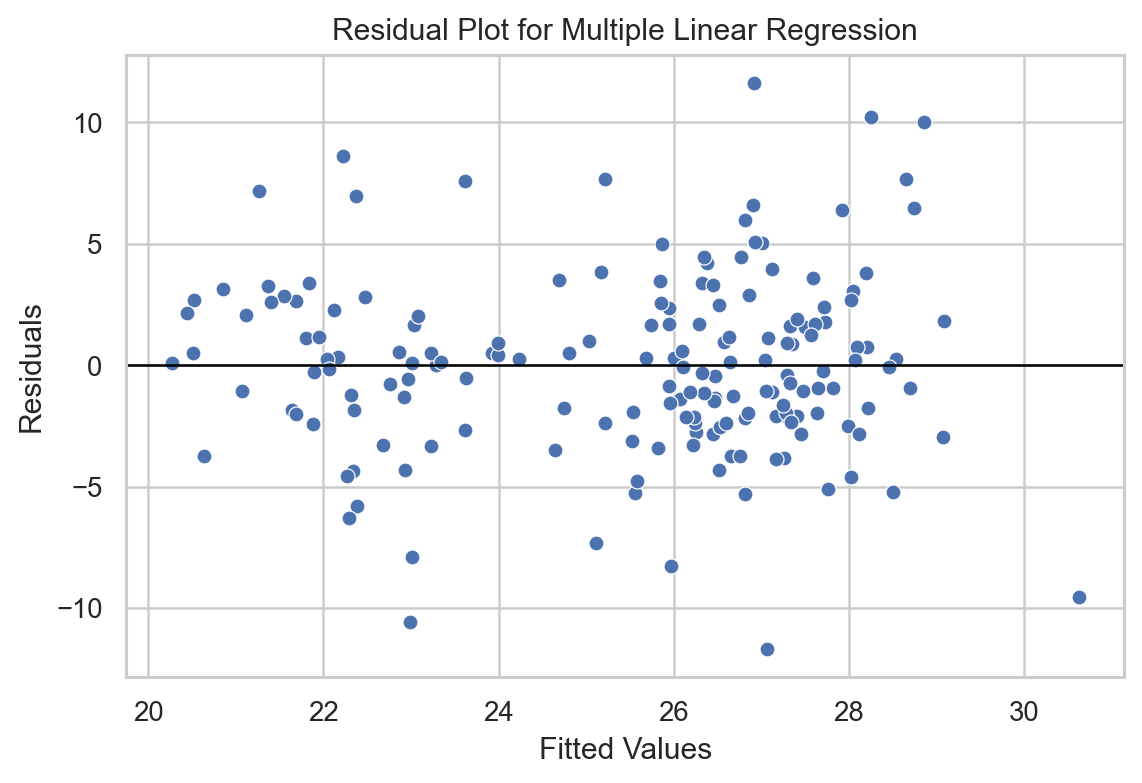
\includegraphics[width=\columnwidth]{../figures/multiple_regression_residuals.png}
\caption{Residual plot for the full multiple linear regression.}
\end{figure}

\begin{figure}[t]
\centering
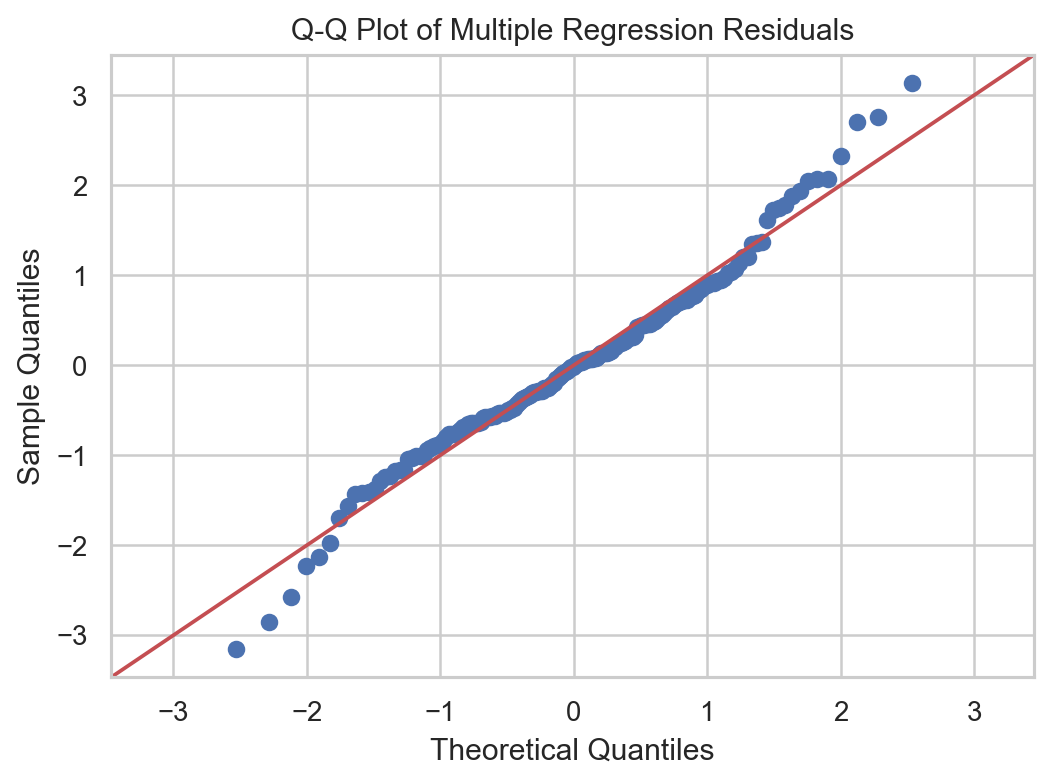
\includegraphics[width=\columnwidth]{../figures/multiple_regression_qq.png}
\caption{Q-Q plot for the full multiple linear regression residuals.}
\end{figure}

\section{First Takeaway}
The most consistent BMI-related variable in this first run is self-reported weight gain. Cycle irregularity showed a BMI difference in the two-sample t-test, but the coefficient became smaller after adjustment. Waist-to-hip ratio, AMH, LH/FSH ratio, random blood sugar, and ultrasound follicle measures did not show strong independent linear associations with BMI in this PCOS-positive subset.

\section{Links to Share}
\begin{itemize}
\item Kaggle dataset: \url{https://www.kaggle.com/datasets/prasoonkottarathil/polycystic-ovary-syndrome-pcos}
\item AutoPCOS paper using clinical/lab/ultrasound blocks: \url{https://www.frontiersin.org/journals/endocrinology/articles/10.3389/fendo.2026.1760541/full}
\item Explainable ML paper using this Kaggle dataset: \url{https://www.mdpi.com/2571-5577/6/2/32}
\item Staged-modeling preprint discussing label limitations: \url{https://www.medrxiv.org/content/10.1101/2025.10.27.25338898v2.full-text}
\item 2023 international PCOS guideline page: \url{https://www.monash.edu/medicine/mchri/pcos/guideline}
\end{itemize}

\begin{thebibliography}{9}
\bibitem{autopcos} Hou et al. AutoPCOS: a stepwise multimodal intelligent framework for polycystic ovary syndrome risk stratification and diagnostic support. \textit{Frontiers in Endocrinology}, 2026.
\bibitem{mdpi} Denny et al. A Distinctive Explainable Machine Learning Framework for Detection of Polycystic Ovary Syndrome. \textit{Applied System Innovation}, 2023.
\bibitem{medrxiv} A Step Toward The Use of AI for Polycystic Ovary Syndrome: Staged Modelling with Uncertainty-Aware Triage and Conformal Prediction with Cost-Efficient Risk. \textit{medRxiv}, 2025.
\end{thebibliography}

\end{document}
